\documentclass{standalone}
\usepackage{tikz}
\usetikzlibrary{patterns, positioning}


\begin{document}
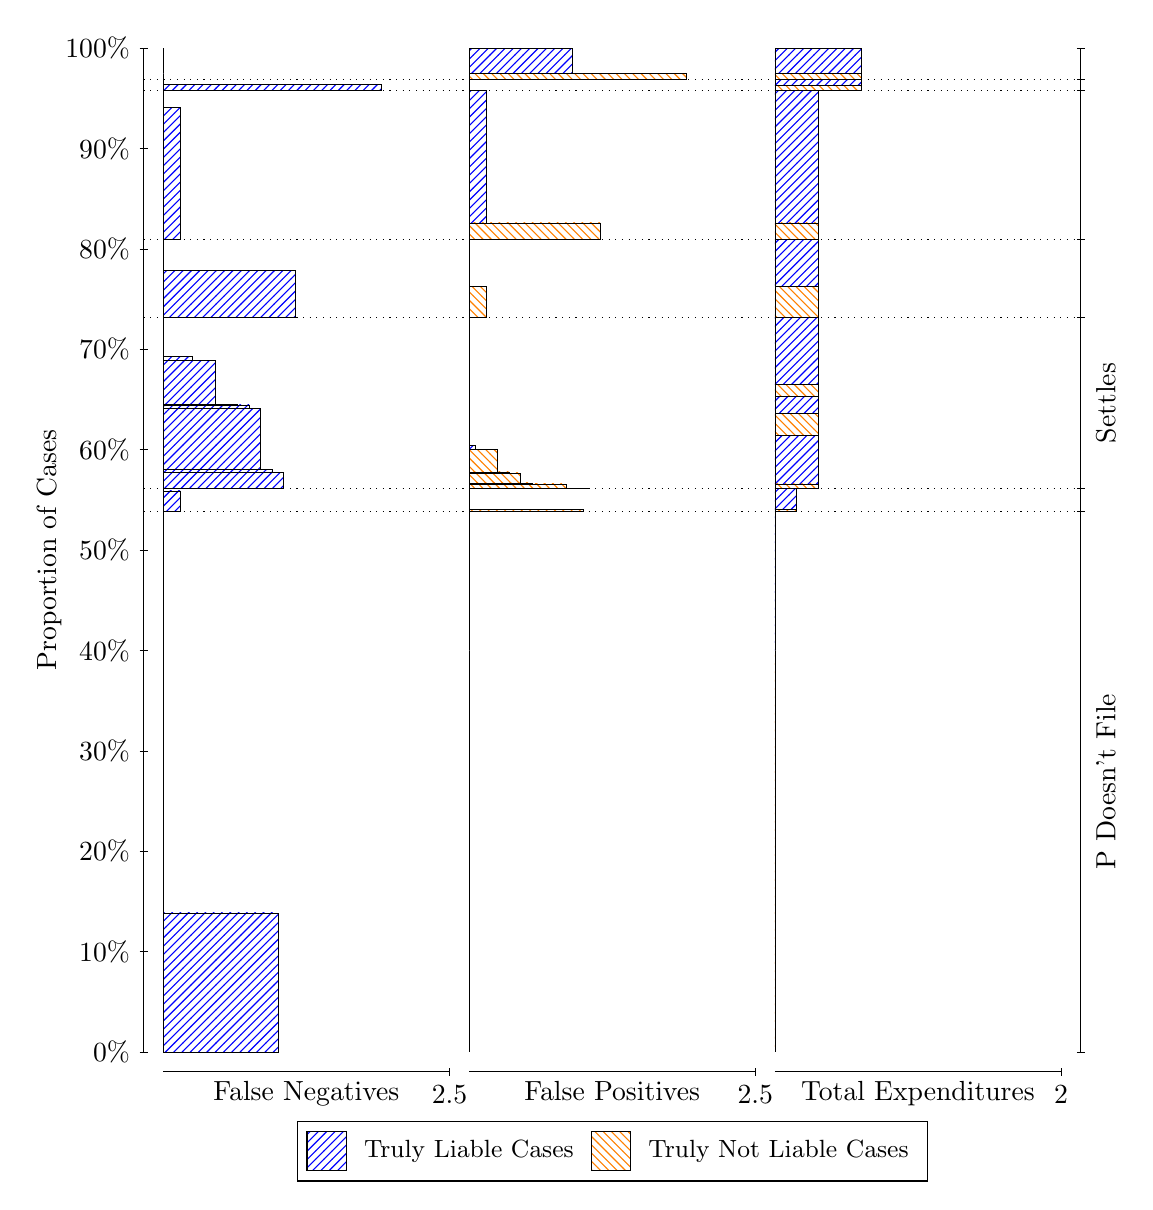
\begin{tikzpicture}
\draw[black, very thin] (1.5,1.75) -- (1.5,14.5);
\node[rotate=90, text=black, anchor=center] at (0.3, 8.125) {Proportion of Cases};
\draw[black, very thin] (1.45,1.75) -- (1.55,1.75);
\node[text=black, anchor=east] at (1.45, 1.75) {0\%};
\draw[black, very thin] (1.45,3.025) -- (1.55,3.025);
\node[text=black, anchor=east] at (1.45, 3.025) {10\%};
\draw[black, very thin] (1.45,4.3) -- (1.55,4.3);
\node[text=black, anchor=east] at (1.45, 4.3) {20\%};
\draw[black, very thin] (1.45,5.575) -- (1.55,5.575);
\node[text=black, anchor=east] at (1.45, 5.575) {30\%};
\draw[black, very thin] (1.45,6.85) -- (1.55,6.85);
\node[text=black, anchor=east] at (1.45, 6.85) {40\%};
\draw[black, very thin] (1.45,8.125) -- (1.55,8.125);
\node[text=black, anchor=east] at (1.45, 8.125) {50\%};
\draw[black, very thin] (1.45,9.4) -- (1.55,9.4);
\node[text=black, anchor=east] at (1.45, 9.4) {60\%};
\draw[black, very thin] (1.45,10.675) -- (1.55,10.675);
\node[text=black, anchor=east] at (1.45, 10.675) {70\%};
\draw[black, very thin] (1.45,11.95) -- (1.55,11.95);
\node[text=black, anchor=east] at (1.45, 11.95) {80\%};
\draw[black, very thin] (1.45,13.225) -- (1.55,13.225);
\node[text=black, anchor=east] at (1.45, 13.225) {90\%};
\draw[black, very thin] (1.45,14.5) -- (1.55,14.5);
\node[text=black, anchor=east] at (1.45, 14.5) {100\%};

\draw[black, very thin] (13.4,1.75) -- (13.4,14.5);
\draw[black, very thin] (13.35,1.75) -- (13.45,1.75);
\node[anchor=west] at (13.35, 1.75) {};
\draw[black, very thin] (13.35,8.6155) -- (13.45,8.6155);
\node[anchor=west] at (13.35, 8.6155) {};
\draw[black, very thin] (13.35,8.9032) -- (13.45,8.9032);
\node[anchor=west] at (13.35, 8.9032) {};
\draw[black, very thin] (13.35,11.081) -- (13.45,11.081);
\node[anchor=west] at (13.35, 11.081) {};
\draw[black, very thin] (13.35,12.07) -- (13.45,12.07);
\node[anchor=west] at (13.35, 12.07) {};
\draw[black, very thin] (13.35,13.96) -- (13.45,13.96);
\node[anchor=west] at (13.35, 13.96) {};
\draw[black, very thin] (13.35,14.104) -- (13.45,14.104);
\node[anchor=west] at (13.35, 14.104) {};
\draw[black, very thin] (13.35,14.5) -- (13.45,14.5);
\node[anchor=west] at (13.35, 14.5) {};

\draw[black, very thin, pattern color=blue, pattern=north east lines] (1.75,1.75) rectangle (3.2033,3.517);
\draw[black, very thin, pattern color=orange, pattern=north west lines] (1.75,3.517) rectangle (1.75,8.6155);
\draw[black, very thin, pattern color=blue, pattern=north east lines] (1.75,8.6155) rectangle (1.968,8.8769);
\draw[black, very thin, pattern color=orange, pattern=north west lines] (1.75,8.8769) rectangle (1.75,8.9032);
\draw[black, very thin, pattern color=blue, pattern=north east lines] (1.75,8.9032) rectangle (3.276,9.1101);
\draw[black, very thin, pattern color=blue, pattern=north east lines] (1.75,9.1101) rectangle (3.1307,9.1485);
\draw[black, very thin, pattern color=blue, pattern=north east lines] (1.75,9.1485) rectangle (2.9853,9.9227);
\draw[black, very thin, pattern color=blue, pattern=north east lines] (1.75,9.9227) rectangle (2.84,9.9676);
\draw[black, very thin, pattern color=blue, pattern=north east lines] (1.75,9.9676) rectangle (2.6947,9.9722);
\draw[black, very thin, pattern color=blue, pattern=north east lines] (1.75,9.9722) rectangle (2.5493,9.9745);
\draw[black, very thin, pattern color=blue, pattern=north east lines] (1.75,9.9745) rectangle (2.404,10.533);
\draw[black, very thin, pattern color=blue, pattern=north east lines] (1.75,10.533) rectangle (2.1133,10.582);
\draw[black, very thin, pattern color=orange, pattern=north west lines] (1.75,10.582) rectangle (1.75,11.081);
\draw[black, very thin, pattern color=blue, pattern=north east lines] (1.75,11.081) rectangle (3.4213,11.674);
\draw[black, very thin, pattern color=orange, pattern=north west lines] (1.75,11.674) rectangle (1.75,12.07);
\draw[black, very thin, pattern color=blue, pattern=north east lines] (1.75,12.07) rectangle (1.968,13.749);
\draw[black, very thin, pattern color=orange, pattern=north west lines] (1.75,13.749) rectangle (1.75,13.96);
\draw[black, very thin, pattern color=blue, pattern=north east lines] (1.75,13.96) rectangle (4.5113,14.034);
\draw[black, very thin, pattern color=orange, pattern=north west lines] (1.75,14.034) rectangle (1.75,14.104);
\draw[black, very thin, pattern color=orange, pattern=north west lines] (1.75,14.104) rectangle (1.75,14.179);
\draw[black, very thin, pattern color=blue, pattern=north east lines] (1.75,14.179) rectangle (1.75,14.5);
\draw[black, very thin, pattern color=orange, pattern=north west lines] (5.6333,1.75) rectangle (5.6333,6.8485);
\draw[black, very thin, pattern color=blue, pattern=north east lines] (5.6333,6.8485) rectangle (5.6333,8.6155);
\draw[black, very thin, pattern color=orange, pattern=north west lines] (5.6333,8.6155) rectangle (7.0867,8.6418);
\draw[black, very thin, pattern color=blue, pattern=north east lines] (5.6333,8.6418) rectangle (5.6333,8.9032);
\draw[black, very thin, pattern color=orange, pattern=north west lines] (5.6333,8.9032) rectangle (7.1593,8.9074);
\draw[black, very thin, pattern color=orange, pattern=north west lines] (5.6333,8.9074) rectangle (6.8687,8.9639);
\draw[black, very thin, pattern color=orange, pattern=north west lines] (5.6333,8.9639) rectangle (6.7233,8.9643);
\draw[black, very thin, pattern color=orange, pattern=north west lines] (5.6333,8.9643) rectangle (6.578,8.9653);
\draw[black, very thin, pattern color=orange, pattern=north west lines] (5.6333,8.9653) rectangle (6.4327,8.978);
\draw[black, very thin, pattern color=orange, pattern=north west lines] (5.6333,8.978) rectangle (6.2873,9.1042);
\draw[black, very thin, pattern color=orange, pattern=north west lines] (5.6333,9.1042) rectangle (6.142,9.118);
\draw[black, very thin, pattern color=orange, pattern=north west lines] (5.6333,9.118) rectangle (5.9967,9.4022);
\draw[black, very thin, pattern color=blue, pattern=north east lines] (5.6333,9.4022) rectangle (5.706,9.451);
\draw[black, very thin, pattern color=blue, pattern=north east lines] (5.6333,9.451) rectangle (5.6333,11.081);
\draw[black, very thin, pattern color=orange, pattern=north west lines] (5.6333,11.081) rectangle (5.8513,11.477);
\draw[black, very thin, pattern color=blue, pattern=north east lines] (5.6333,11.477) rectangle (5.6333,12.07);
\draw[black, very thin, pattern color=orange, pattern=north west lines] (5.6333,12.07) rectangle (7.3047,12.28);
\draw[black, very thin, pattern color=blue, pattern=north east lines] (5.6333,12.28) rectangle (5.8513,13.96);
\draw[black, very thin, pattern color=orange, pattern=north west lines] (5.6333,13.96) rectangle (5.6333,14.03);
\draw[black, very thin, pattern color=blue, pattern=north east lines] (5.6333,14.03) rectangle (5.6333,14.104);
\draw[black, very thin, pattern color=orange, pattern=north west lines] (5.6333,14.104) rectangle (8.3947,14.179);
\draw[black, very thin, pattern color=blue, pattern=north east lines] (5.6333,14.179) rectangle (6.9413,14.5);
\draw[black, very thin, pattern color=orange, pattern=north west lines] (9.5167,1.75) rectangle (9.5167,6.8485);
\draw[black, very thin, pattern color=blue, pattern=north east lines] (9.5167,6.8485) rectangle (9.5167,8.6155);
\draw[black, very thin, pattern color=orange, pattern=north west lines] (9.5167,8.6155) rectangle (9.7892,8.6418);
\draw[black, very thin, pattern color=blue, pattern=north east lines] (9.5167,8.6418) rectangle (9.7892,8.9032);
\draw[black, very thin, pattern color=orange, pattern=north west lines] (9.5167,8.9032) rectangle (10.062,8.9653);
\draw[black, very thin, pattern color=blue, pattern=north east lines] (9.5167,8.9653) rectangle (10.062,9.5797);
\draw[black, very thin, pattern color=orange, pattern=north west lines] (9.5167,9.5797) rectangle (10.062,9.864);
\draw[black, very thin, pattern color=blue, pattern=north east lines] (9.5167,9.864) rectangle (10.062,10.071);
\draw[black, very thin, pattern color=orange, pattern=north west lines] (9.5167,10.071) rectangle (10.062,10.224);
\draw[black, very thin, pattern color=blue, pattern=north east lines] (9.5167,10.224) rectangle (10.062,11.081);
\draw[black, very thin, pattern color=orange, pattern=north west lines] (9.5167,11.081) rectangle (10.062,11.477);
\draw[black, very thin, pattern color=blue, pattern=north east lines] (9.5167,11.477) rectangle (10.062,12.07);
\draw[black, very thin, pattern color=orange, pattern=north west lines] (9.5167,12.07) rectangle (10.062,12.28);
\draw[black, very thin, pattern color=blue, pattern=north east lines] (9.5167,12.28) rectangle (10.062,13.96);
\draw[black, very thin, pattern color=orange, pattern=north west lines] (9.5167,13.96) rectangle (10.607,14.03);
\draw[black, very thin, pattern color=blue, pattern=north east lines] (9.5167,14.03) rectangle (10.607,14.104);
\draw[black, very thin, pattern color=orange, pattern=north west lines] (9.5167,14.104) rectangle (10.607,14.179);
\draw[black, very thin, pattern color=blue, pattern=north east lines] (9.5167,14.179) rectangle (10.607,14.5);
\draw[black, dotted] (1.5,8.6155) -- (13.4,8.6155);
\draw[black, dotted] (1.5,8.9032) -- (13.4,8.9032);
\draw[black, dotted] (1.5,11.081) -- (13.4,11.081);
\draw[black, dotted] (1.5,12.07) -- (13.4,12.07);
\draw[black, dotted] (1.5,13.96) -- (13.4,13.96);
\draw[black, dotted] (1.5,14.104) -- (13.4,14.104);
\draw[black, very thin] (1.75,1.5) -- (5.3833,1.5);
\node[text=black, anchor=north] at (3.5667, 1.5) {False Negatives};
\draw[black, very thin] (5.3833,1.45) -- (5.3833,1.55);
\node[text=black, anchor=north] at (5.3833, 1.45) {2.5};

\draw[black, very thin] (5.6333,1.5) -- (9.2667,1.5);
\node[text=black, anchor=north] at (7.45, 1.5) {False Positives};
\draw[black, very thin] (9.2667,1.45) -- (9.2667,1.55);
\node[text=black, anchor=north] at (9.2667, 1.45) {2.5};

\draw[black, very thin] (9.5167,1.5) -- (13.15,1.5);
\node[text=black, anchor=north] at (11.333, 1.5) {Total Expenditures};
\draw[black, very thin] (13.15,1.45) -- (13.15,1.55);
\node[text=black, anchor=north] at (13.15, 1.45) {2};

\node[text=black, centered, rotate=90] at (13.72, 5.1828) {P Doesn't File};

\node[text=black, centered, rotate=90] at (13.72, 9.9921) {Settles};





\draw (7.449999999999999,1.5) node[draw=none] (baseCoordinate) {};
\begin{scope}[align=center]
        \matrix[scale=0.5, draw=black, below=0.5cm of baseCoordinate, nodes={draw}, column sep=0.1cm]{
            \node[rectangle, draw, minimum width=0.5cm, minimum height=0.5cm, pattern color=blue, pattern=north east lines] {}; &
            \node[draw=none, font=\small, text=black] (B) {Truly Liable Cases}; &
            \node[rectangle, draw, minimum width=0.5cm, minimum height=0.5cm, pattern color=orange, pattern=north west lines] {}; &
            \node[draw=none, font=\small, text=black] (B) {Truly Not Liable Cases}; \\
            };
\end{scope}

\end{tikzpicture}
\end{document}